% Template Taken from NIPS 2012
%
% Document Properties
\documentclass[fleqn]{article}
\usepackage{nips12submit_e,times}
%
% Inserted Packages (Gregory Added)
\usepackage{enumerate}
\usepackage{appendix}
\usepackage{float}
\usepackage{amsmath}
\usepackage{algorithm, algorithmic}
\usepackage{amsfonts}%
\usepackage{amssymb}%
\usepackage{graphicx}
%
%-------------------------------------------------------------------------------
\title{Prediction of Chess Endgame using\\
Decision Tree and SVM Classifiers}

\author{
Anderson, Michael\\
CS\\ 
\texttt{andermic@eecs.oregonstate.edu} \\
\AND
Gutshall, Gregory\\
ECE\\
\texttt{gutshalg@eecs.oregonstate.edu} \\
}

\newcommand{\fix}{\marginpar{FIX}}
\newcommand{\new}{\marginpar{NEW}}

\nipsfinalcopy % Uncomment for camera-ready version

\begin{document}

\maketitle

\begin{abstract}
Insert Abstract Text Here.
\end{abstract}

% ***********************************************
\section{Introduction}
\label{sec:Intro}
%
\subsection[Background]{Background\textbackslash Problem Formulation}
\label{subsec:Background}
Discuss what a Chess Endgame is.  Discuss how one would go about determining a Chess Endgame?  
%
\subsection{Outline of Report}
\label{subsec:outline}
In section(\ref{sec:Dataset}) we describe the dataset from the UCI repository used for our training and testing environment.  We also provide insight into the parameterizations of the original data and why we think those parameterizations will yield improved classification results.  In section(\ref{sec:Theory}) we discuss the theory and limitations of the two proposed classification methods.  In section(\ref{sec:Results}) we will show results heuristically drawn from simulations for the two proposed methods and discuss results related to these findings.  Finally, in section(\ref{sec:Conclusions}) we will make final conclusions and possible algorithmic strategies to improve the results. 

% ***********************************************
\section{Dataset}
\label{sec:Dataset}

\subsection{Chess (King-Rook vs. King) Data Set}
\label{subsec:dataset}
Discuss the dataset from UCI.  Format of the data.

\subsubsection{Notation}

\paragraph{Chess Board Positions:}
Let the following notation describe the space of a Chess board,
\begin{equation}
\label{eq:StandardPositions}
\begin{aligned}
	\text{File} &\in \left[a,b,c,d,e,f,g,h\right]\\
	&\in \left[1,2,3,4,5,6,7,8\right]\\
	\text{Rank} &\in \left[1,2,3,4,5,6,7,8\right]\\
\end{aligned}
\end{equation}

\paragraph{Game Pieces:}
Let the three game pieces be defined as $Piece_i$, where $i = \left[1,2,3\right]$ represents the piece index,
\begin{equation}
\label{eq:pieces}
\begin{aligned}
	Piece &\in \left[W_k, W_r, B_k\right]\\
	&W_k = \text{White King}\\
	&W_r = \text{White Rook}\\
	&B_k = \text{Black King}\\
\end{aligned}
\end{equation}

\paragraph{Examples:}
Let a example of a game be defined as $Game_j$ where $j = \left[1,2,3,\dots\right]$ is the game row index, 
%
\begin{equation}
\begin{aligned}
	Game_j &= \left[Piece_i \left\{file_j, rank_j\right\}\right]\\
\end{aligned}
\end{equation}
%
The entire set of examples is labeled as $\mathbf{X}$.

\paragraph{Class Labels:}
Class labels are defined as the remaining moves till checkmate of $B_k$.  Note, checkmate of $B_k$ is called on the $m^{\text{th}}$ move of $B_k$.
\begin{equation}
\begin{aligned}
	y_j &\in \left[draw,0,1,2,3,4, \dots, m\right]\\
	&\in \left[-1,0,1,2,3,4, \dots, m\right]
\end{aligned}
\end{equation}
%
The entire set of training class labels is labeled as $\mathbf{y}$.

\subsection{Parameterization}
\label{subsec:Parameterization}
Discuss how we parameterized the data.

Several parameter functions are used to classify or achieve an objective function, these parameter functions are labeled as $\mathbf{\Phi}\left(\mathbf{X}\right)$. 

% ***********************************************
\section{Theory of Proposed Methods}
\label{sec:Theory}

\subsection{Theory: Decision Trees}
\label{sub:theoryDecisionTrees}
Theory goes here.

\subsection{Theory: Support Vector Machines (SVM)}
\label{sub:theorySVM}
Theory goes here.

% ***********************************************
\section[Results]{Simulation\textbackslash Classification Results}
\label{sec:Results}

\subsection{Results: Decision Tree}
\label{sub:resultsTrees}

\subsection{Results: Support Vector Machine (SVM)}
\label{sub:resultsSVM}
You can insert images by using the following code.  Just place them in the figs folder and make sure they are in *.eps format.\cite{bishop:2006}
%
\begin{figure}[H]
	{\centering
		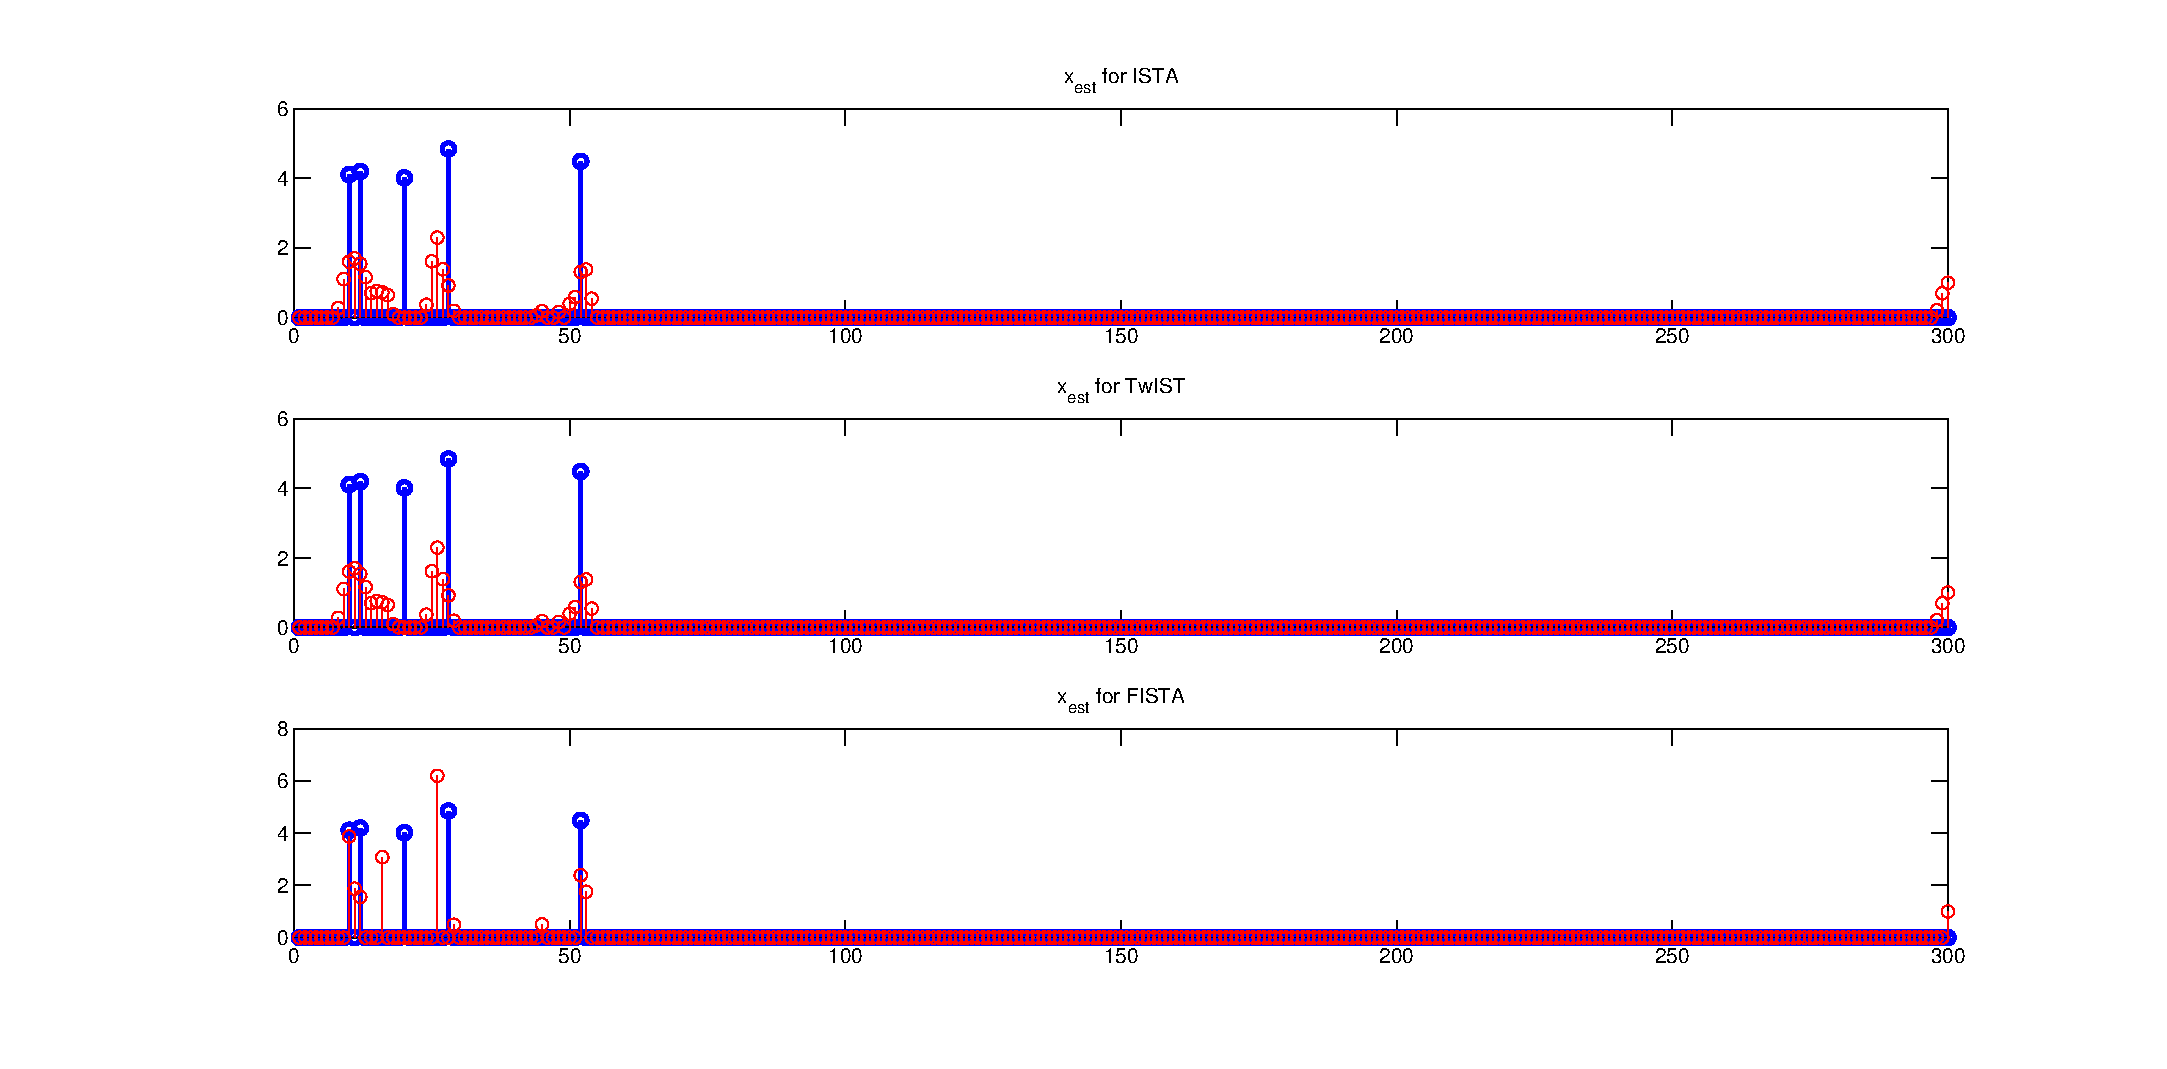
\includegraphics[trim = 10mm 10mm 10mm 0mm, clip,width=1.0\textwidth]{figs/Test_Image}
		\caption{CaptionName: Test Image from figs folder}
		\label{fig:Test}
	}
\end{figure}

% ***********************************************
\section{Conclusions}
\label{sec:Conclusions}

% ***********************************************
\nocite{*}  %Uncomment this line to print all citations 
\bibliographystyle{IEEEbib}
\bibliography{references} 

\end{document}